\documentclass{article}
\usepackage[lastexercise]{exercise} %answerdelayed
\usepackage{calc}
\setcounter{tocdepth}{2}
\providecommand{\keywords}[1]{\textbf{\textit{Keywords---}} #1}
\usepackage{tikz-cd}
\usepackage{tensor}
% \usepackage{hyperref}
% \usepackage{csquotes}
\usepackage{fancyvrb}
\usepackage{todonotes}
\usepackage{verbatim}
\usepackage{amsmath}
\usepackage{microtype}
\usepackage{amssymb}
\usepackage{amsthm}
\usepackage{thmtools}
\usepackage{nameref,hyperref}
\usepackage{cleveref}
\usepackage[utf8]{inputenc}

\setcounter{tocdepth}{5}

\newcommand{\ts}[2]{{_{#1}}\!\!\times_{#2}\!}
\newcommand{\tens}[2]{{_{#1}}\times_{#2}}

\declaretheorem[numberwithin=section]{theorem}
\declaretheorem[sibling=theorem]{exercise}
\declaretheorem[sibling=theorem]{example}
\declaretheorem[sibling=theorem]{non-example}
\declaretheorem[sibling=theorem]{lemma}
\declaretheorem[sibling=theorem]{corollary}
\declaretheorem[sibling=theorem]{proposition}
\declaretheorem[style=definition,sibling=theorem]{definition}
\declaretheorem[style=definition,sibling=theorem]{axiom}
\declaretheorem[style=definition,sibling=theorem]{notation}
\declaretheorem[sibling=theorem]{question}
\declaretheorem[style=remark,sibling=theorem]{remark}
\title{Worked Examples}
\author{Work in progress}
\begin{document}
\maketitle
\tableofcontents

\begin{Exercise}
  Suppose that the internet consists of three pages $P_1$, $P_2$ and $P_3$.
  Suppose further that:-
  \begin{itemize}
    \item there are two links from $P_1$ to $P_2$
    \item there is one link from $P_1$ to $P_3$
    \item there is one link from $P_2$ to $P_1$
    \item there is one link from $P_2$ to $P_3$
    \item there is one link from $P_3$ to $P_2$
  \end{itemize}
  Then calculate the (relative) PageRanks for $P_1$, $P_2$ and $P_3$.
\end{Exercise}

\begin{Answer}
  The transition matrix is:
  \begin{equation*}
  \left[
  \begin{matrix}
  0 & \frac{1}{2} & 0\\
  \frac{2}{3} & 0 & 1\\
  \frac{1}{3} & \frac{1}{2} & 0
  \end{matrix}
  \right]
  \end{equation*}
  So we get the steady state vector by solving $(A-I)v = 0$:
  \begin{equation*}
  \left[
  \begin{array}{ccc|c}
  -1 & \frac{1}{2} & 0 & 0\\
  \frac{2}{3} & -1 & 1 & 0\\
  \frac{1}{3} & \frac{1}{2} & -1 & 0 
  \end{array}
  \right]
  \end{equation*}
  \begin{equation*}
  \left[
  \begin{array}{ccc|c}
  1 & \frac{-1}{2} & 0 & 0\\
  2 & -3 & 3 & 0\\
  1 & \frac{3}{2} & -3 & 0 
  \end{array}
  \right]
  \end{equation*}
  \begin{equation*}
  \left[
  \begin{array}{ccc|c}
  1 & \frac{-1}{2} & 0 & 0\\
  0 & -2 & 3 & 0\\
  0 & 2 & -3 & 0 
  \end{array}
  \right]
  \end{equation*}
  \begin{equation*}
  \left[
  \begin{array}{ccc|c}
  1 & \frac{-1}{2} & 0 & 0\\
  0 & 1 & \frac{-3}{2} & 0 
  \end{array}
  \right]
  \end{equation*}
    \begin{equation*}
  \left[
  \begin{array}{ccc|c}
  1 & 0 & \frac{-3}{4} & 0\\
  0 & 1 & \frac{-3}{2} & 0 
  \end{array}
  \right]
  \end{equation*}
  so $z = s$, $x = \frac{3s}{4}$ and $y = \frac{3s}{2}$.
  So the eigenspace associated to the eigenvalue $1$ is:
  \begin{equation*}
  E_1 = s \left[
  \begin{array}{c}
  \frac{3}{4}\\
  \frac{3}{2}\\
  1
  \end{array}
  \right] = \bar{s} \left[
  \begin{array}{c}
  3\\
  6\\
  4
  \end{array}
  \right]
  \end{equation*}
  and so the steady state vector (containing the PageRanks) is
  \begin{equation*}
  \frac{1}{13}
  \left[
  \begin{array}{c}
  3\\
  6\\
  4
  \end{array}
  \right]
  \end{equation*}
  because we need to choose $\bar{s}$ so that the sum of the entries is $1$.
\end{Answer}

\begin{Exercise}
  Find the distance $\alpha$ between the lines
\begin{equation*}
L_1: \vec{x} = \left[
\begin{matrix}
-6\\
-7\\
7
\end{matrix}
\right]+s
\left[
\begin{matrix}
2\\
1\\
-1
\end{matrix}
\right] = P+sd
\end{equation*}
and
\begin{equation*}
L_2: \vec{x} =
\left[
\begin{matrix}
-7\\
-14\\
0
\end{matrix}
\right]+ t \left[
\begin{matrix}
2\\
3\\
-1
\end{matrix}
\right] = Q + te
\end{equation*}
and find a points $A$ on $L_1$ and $B$ on $L_2$ such that $dist(A, B) = \alpha$.
\end{Exercise}

\begin{Answer}
First draw the picture:\\

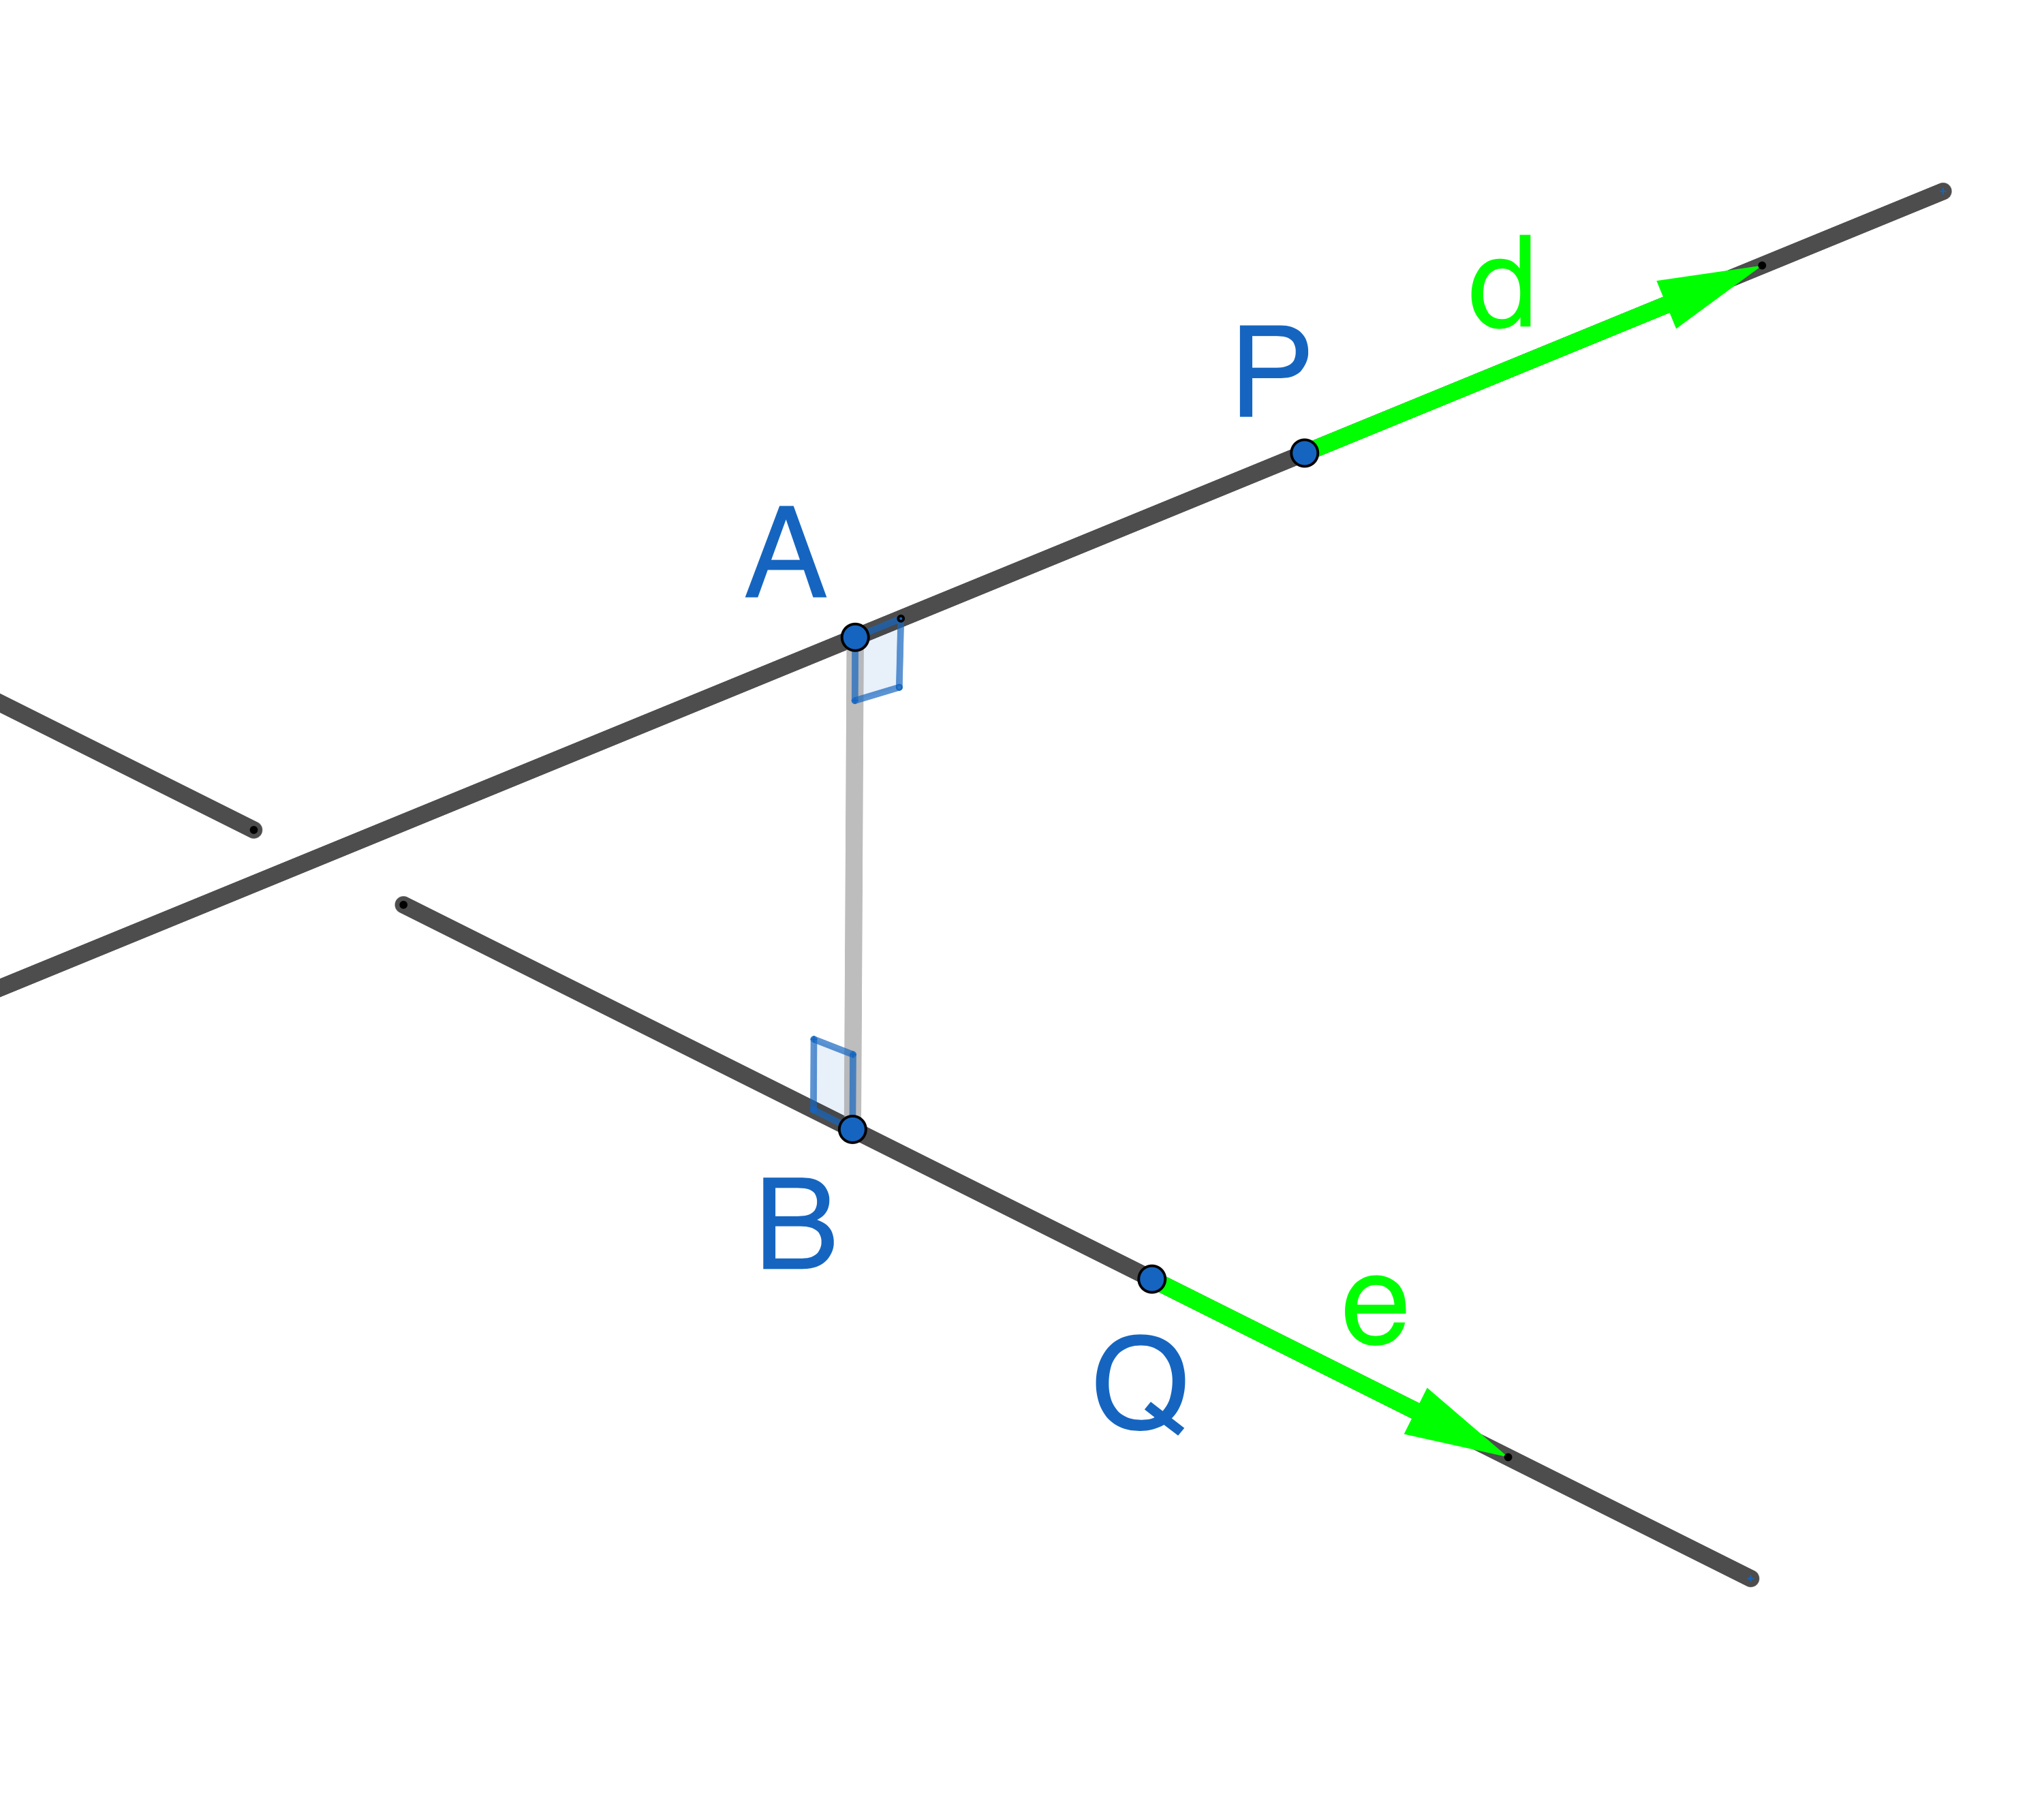
\includegraphics[scale=0.3]{skew-lines.png}

where we want to find $A$ and $B$.
Since $\vec{AB}$ is orthogonal to both $d$ and $e$:
\begin{equation}\label{othog-eqns}
  (B-A)\cdot d = 0 \text{ and }
  (B-A)\cdot e = 0
\end{equation}
First we can express $B-A$ in terms of unknowns $s$ and $t$:
\begin{equation*}
B-A = \left[
\begin{array}{c}
-7+2t\\
-14+3t\\
-t
\end{array}
\right] - \left[
\begin{array}{c}
-6+2s\\
-7 +s\\
7-s
\end{array}
\right] = 
\left[
\begin{array}{c}
2t-2s-1\\
3t-s-7\\
-t+s-7
\end{array}
\right]
\end{equation*}
because $A$ is on $L_1$ and $B$ is on $L_2$. Then \ref{othog-eqns} gives firstly:
\begin{align*}
0 &= \left[
\begin{array}{c}
2t-2s-1\\
3t-s-7\\
-t+s-7
\end{array}
\right]\cdot \left[
\begin{array}{c}
2\\
1\\
-1
\end{array}
\right] \\
&= 4t-4s-2 +3t-s-7+t-s+7\\
&= 8t -6s -2
\end{align*}
and secondly
\begin{align*}
0 &= \left[
\begin{array}{c}
2t-2s-1\\
3t-s-7\\
-t+s-7
\end{array}
\right]\cdot \left[
\begin{array}{c}
2\\
3\\
-1
\end{array}
\right] \\
&= 4t-4s-2+9t-3s-21+t-s+7\\
&= 14t -8s -16
\end{align*}
Next find $t$ and $s$ by solving
\begin{equation*}
\left[
\begin{array}{cc|c}
8 & -6 & 2\\
14 & -8 & 16
\end{array}
\right]
\end{equation*}
\begin{equation*}
\left[
\begin{array}{cc|c}
1 & \frac{-3}{4} & \frac{1}{4}\\
7 & -4 & 8
\end{array}
\right]
\end{equation*}
\begin{equation*}
\left[
\begin{array}{cc|c}
1 & \frac{-3}{4} & \frac{1}{4}\\
0 & \frac{5}{4} & \frac{25}{4}
\end{array}
\right]
\end{equation*}
\begin{equation*}
\left[
\begin{array}{cc|c}
1 & \frac{-3}{4} & \frac{1}{4}\\
0 & 1 & 5
\end{array}
\right]
\end{equation*}
\begin{equation*}
\left[
\begin{array}{cc|c}
1 & 0 & 4\\
0 & 1 & 5
\end{array}
\right]
\end{equation*}
so $t = 4$ and $s = 5$.
Therefore
\begin{equation*}
A = P+sd = \left[
\begin{array}{c}
-6\\
-7\\
7
\end{array}
\right] + 5 \left[
\begin{array}{c}
2\\
1\\
-1
\end{array}
\right] = \left[
\begin{array}{c}
4\\
-2\\
2
\end{array}
\right]
\end{equation*}
and 
\begin{equation*}
B = Q+te = \left[
\begin{array}{c}
-7\\
-14\\
0
\end{array}
\right]+4 \left[
\begin{array}{c}
2\\
3\\
-1
\end{array}
\right] = \left[
\begin{array}{c}
1\\
-2\\
-4
\end{array}
\right]
\end{equation*}
so the distance between the lines is:
\begin{equation*}
dist(A, B) = \sqrt{3^2+0^2 + 6^2} = \sqrt{45} = 3\sqrt{5}
\end{equation*}
\end{Answer}

\begin{Exercise}
  Suppose that the sequence $x_0$, $x_1$, $x_2$ \dots is defined by $x_0 = 2$, $x_1 = 1+i$ and $x_{k+2} = (1+i)x_{k+1}-ix_k$. Find a formula for $x_k$.
\end{Exercise}

\begin{Answer}
  Reformulate as a two dimensional discrete linear dynamical system. Let:
  \begin{equation*}
  v_k = \left[
  \begin{array}{c}
  x_{k+1}\\
  x_k
  \end{array}
  \right]\end{equation*}
  and so
  \begin{equation*}
  v_{k+1} = \left[
  \begin{array}{c}
  x_{k+2}\\
  x_{k+1}
  \end{array}
  \right] = \left[
  \begin{array}{cc}
  1+i & -i\\
  1 & 0
  \end{array}
  \right] \left[
  \begin{array}{c}
  x_{k+1}\\
  x_k
  \end{array}
  \right] = Av_{k}
  \end{equation*}
  and
  \begin{equation*}
  v_0 = \left[
  \begin{array}{c}
  x_1\\
  x_0
  \end{array}
  \right] = \left[
  \begin{array}{c}
  1+i\\
  2
  \end{array}
  \right]
  \end{equation*}
  First find the eigenvalues:
  \begin{align*}
  det \left[
  \begin{array}{cc}
  1+i-\lambda & -i\\
  1 & -\lambda
  \end{array}
  \right] &= -\lambda(1+i-\lambda) +i\\
  &= \lambda^2 - (1+i)\lambda +i\\
  &= (\lambda -1)(\lambda -i)
  \end{align*}
  The eigenspace associated to the eigenvalue $1$:
  \begin{equation*}
  \left[
  \begin{array}{cc|c}
  i&-i&0\\
  1&-1&0
  \end{array}
  \right]
  \end{equation*}
  \begin{equation*}
  \rightarrow\left[
  \begin{array}{cc|c}
  1&-1&0
  \end{array}
  \right]
  \end{equation*}
  so $y=s$ and $x = s$ and so the eigenspace is
  \begin{equation*}
  E_1 = s \left[
  \begin{array}{c}
  1\\
  1
  \end{array}
  \right]
  \end{equation*}
  The eigenspace associated to the eigenvalue $i$:
  \begin{equation*}
  \left[
  \begin{array}{cc|c}
  1&-i&0\\
  1&-i&0
  \end{array}
  \right]
  \end{equation*}
  \begin{equation*}
  \rightarrow\left[
  \begin{array}{cc|c}
  1&-i&0\\
  \end{array}
  \right]
  \end{equation*}
  so $y = s$ and $x = is$ and the eigenspace is:
  \begin{equation*}
  E_i = s \left[
  \begin{array}{c}
  i\\
  1
  \end{array}
  \right]
  \end{equation*}
  Next write the initial vector in terms of the eigenvectors:
  \begin{equation*}
  v_0 = \left[
  \begin{array}{c}
  1+i\\
  2
  \end{array}
  \right] = \left[
  \begin{array}{c}
  1\\
  1
  \end{array}
  \right] + \left[
  \begin{array}{c}
  i\\
  1
  \end{array}
  \right]
  \end{equation*}
  to deduce that 
  \begin{align*}
  A^k v_0 &= A^k \left( \left[
  \begin{array}{c}
  1\\
  1
  \end{array}
  \right] + \left[
  \begin{array}{c}
  i\\
  1
  \end{array}
  \right]\right) \\
  &= A^k \left[
  \begin{array}{c}
  1\\
  1
  \end{array}
  \right]+ A^k \left[
  \begin{array}{c}
  i\\
  1
  \end{array}
  \right] \\
  &= \left[
  \begin{array}{c}
  1\\
  1
  \end{array}
  \right] + i^k \left[
  \begin{array}{c}
  i\\
  1
  \end{array}
  \right]
  \end{align*}
  therefore $x_k = 1+i^k$.
\end{Answer}

\begin{Exercise}
  A tennis club organises its games over the course of a year as follows:-
  \begin{itemize}
    \item At the beginning of the year there is a qualifying tournament.
    \item Those who finish in the top half of the qualifying tournament enter league $A$ and those who do not enter league $B$.
    \item Players in both leagues play matches weekly.
    \item Adam joins at the beginning of one year:-
    \begin{itemize}
      \item Adam has probability $\frac{2}{3}$ of finishing in the top half of the qualifying tournament.
      \item In league $A$ Adam has a $\frac{2}{5}$ chance of winning each weekly match.
      \item In league $B$ Adam has a $\frac{4}{5}$ chance of winning each weekly match.
    \end{itemize}
  \end{itemize}
  Model Adam's progress as a Markov chain and find all steady state vectors.
\end{Exercise}

\begin{Answer}
  Let the states be:-
  \begin{itemize}
    \item State 1: Before the qualifying tournament.
    \item State 2: Adam is in league A and won the previous game.
    \item State 3: Adam is in league A and lost the previous game.
    \item State 4: Adam is in league B and won the previous game.
    \item State 5: Adam is in league B and lost the previous game.
  \end{itemize}
  The transition matrix is 
  \begin{equation*}
  \left[
  \begin{array}{ccccc}
  0&0&0&0&0\\
  \frac{2}{3} & \frac{2}{5} & \frac{2}{5} & 0&0\\
  0 & \frac{3}{5} & \frac{3}{5} & 0 & 0\\
  0&0&0 &\frac{4}{5} & \frac{4}{5}\\
  \frac{1}{3} & 0 & 0 & \frac{1}{5} & \frac{1}{5}
  \end{array}
  \right]
  \end{equation*}
  (Notice how the Markov chain splits into two $2\times 2$ blocks after the first iteration.)
  To find the steady state vector we solve:
  \begin{equation*}
  \left[
  \begin{array}{ccccc|c}
  -1&0&0&0&0&0\\
  \frac{2}{3} & \frac{-3}{5} & \frac{2}{5} & 0&0&0\\
  0 & \frac{3}{5} & \frac{-2}{5} & 0 & 0&0\\
  0&0&0 &\frac{-1}{5} & \frac{4}{5}&0\\
  \frac{1}{3} & 0 & 0 & \frac{1}{5} & \frac{-4}{5}&0
  \end{array}
  \right]
  \end{equation*}
  \begin{equation*}
  \rightarrow\left[
  \begin{array}{ccccc|c}
  1&0&0&0&0&0\\
  0 & \frac{-3}{5} & \frac{2}{5} & 0&0&0\\
  0 & \frac{3}{5} & \frac{-2}{5} & 0 & 0&0\\
  0&0&0 &\frac{-1}{5} & \frac{4}{5}&0\\
  0 & 0 & 0 & \frac{1}{5} & \frac{-4}{5}&0
  \end{array}
  \right]
  \end{equation*}
  \begin{equation*}
  \rightarrow\left[
  \begin{array}{ccccc|c}
  1&0&0&0&0&0\\
  0 & \frac{3}{5} & \frac{-2}{5} & 0 & 0&0\\
  0 & 0 & 0 & \frac{1}{5} & \frac{-4}{5}&0
  \end{array}
  \right]
  \end{equation*}
  \begin{equation*}
  \rightarrow\left[
  \begin{array}{ccccc|c}
  1&0&0&0&0&0\\
  0 & 3 & -2 & 0 & 0&0\\
  0 & 0 & 0 & 1 & -4&0
  \end{array}
  \right]
  \end{equation*}
  so $x_3 = s$, $x_5 = t$, $x_1 = 0$, $x_2 = \frac{2s}{3}$ and $x_4 = 4t$.
  Therefore the eigenspace associated to eigenvalue $1$ is:
  \begin{equation*}
  E_1 = \left[
  \begin{array}{c}
  0\\
  \frac{2s}{3}\\
  s\\
  4t\\
  t
  \end{array}
  \right] = s \left[
  \begin{array}{c}
  0\\
  2\\
  3\\
  0\\
  0
  \end{array}
  \right] + t \left[
  \begin{array}{c}
  0\\
  0\\
  0\\
  4\\
  1
  \end{array}
  \right]
  \end{equation*}
  and so there are two steady state vectors:
  \begin{equation}
    \frac{1}{5} \left[
    \begin{array}{c}
    0\\
    2\\
    3\\
    0\\
    0
    \end{array}
    \right] \text{ and }
    \frac{1}{5}\left[
    \begin{array}{c}
    0\\
    0\\
    0\\
    4\\
    1
    \end{array}
    \right]
  \end{equation}
\end{Answer}

\begin{Exercise}
  Find equations for the lines through
  \begin{equation*}
  Q = \left[
  \begin{matrix}
  1\\
  0\\
  1
  \end{matrix}
  \right]
  \end{equation*}
  that meet the line
  \begin{equation*}
  \vec{x} = \left[
  \begin{matrix}
  1\\
  2\\
  0
  \end{matrix}
  \right]+s \left[
  \begin{matrix}
  2\\
  -1\\
  2
  \end{matrix}
  \right] = P+sd
  \end{equation*}
  at the two points at distance $3$ from 
  \begin{equation*}
  P=\left[
  \begin{matrix}
  1\\
  2\\
  0
  \end{matrix}
  \right]
  \end{equation*}
\end{Exercise}

\begin{Answer}
  First draw the picture:\\

  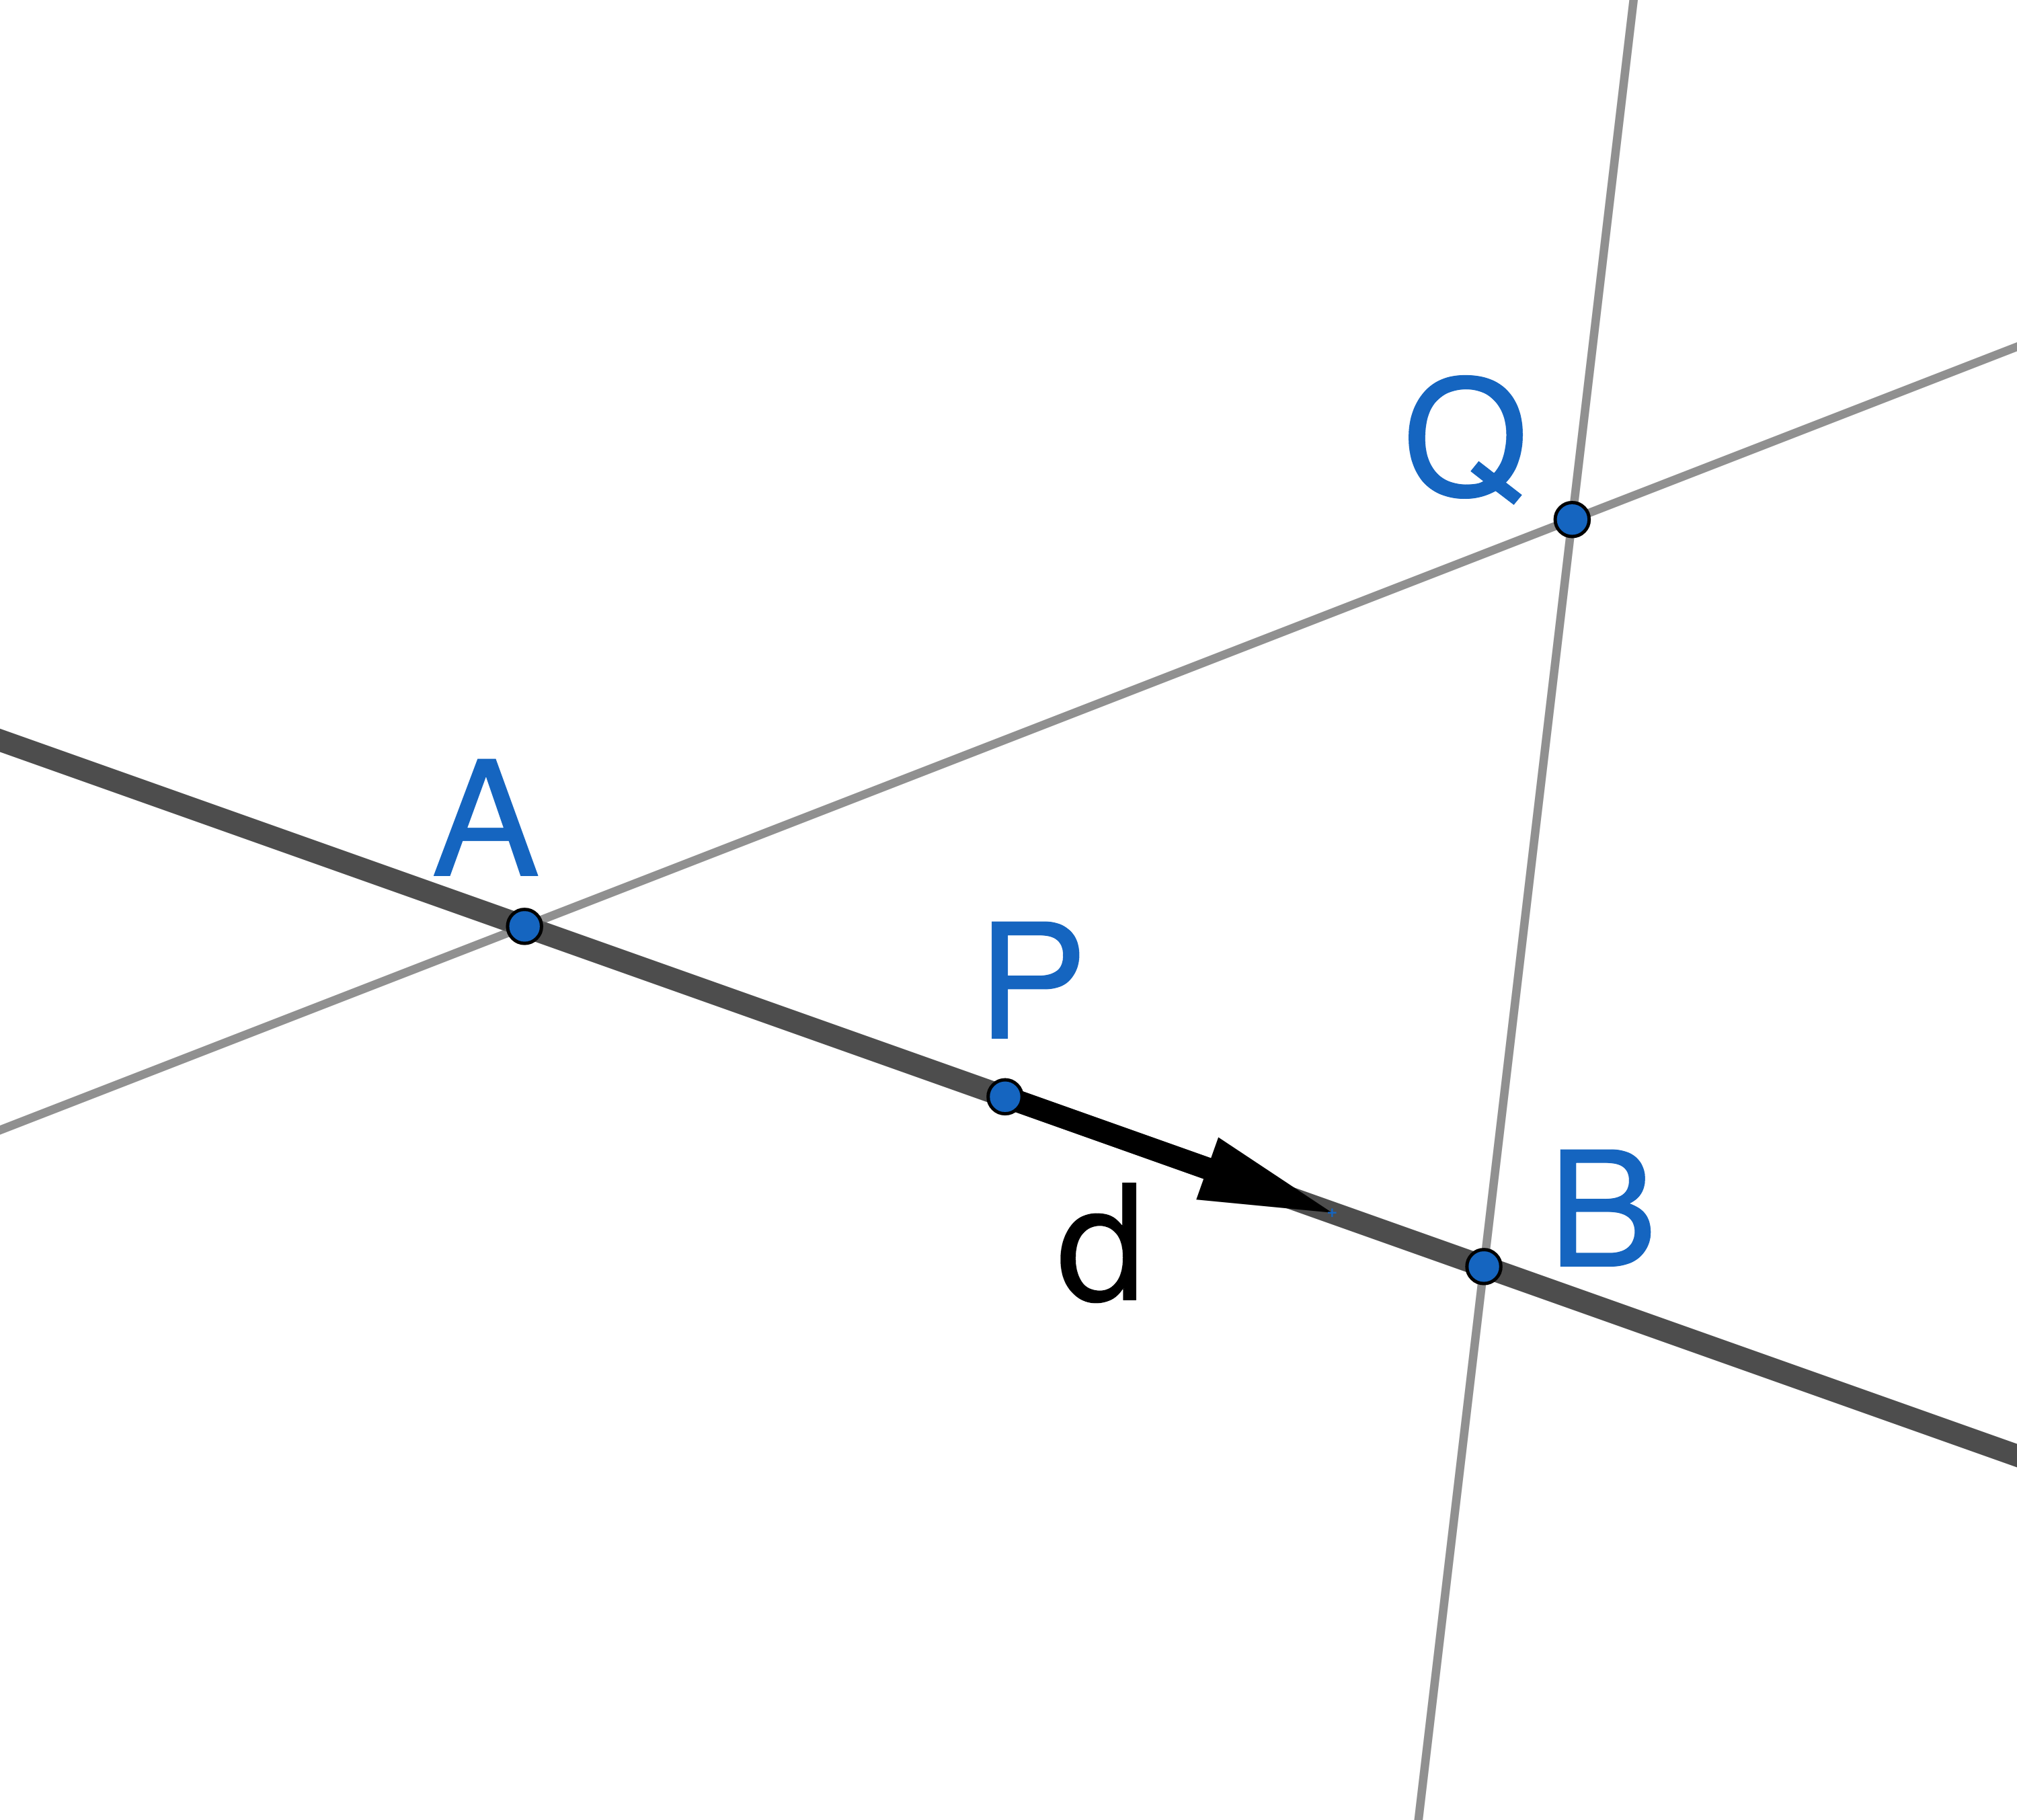
\includegraphics[scale=0.5]{lines-pt-at-dist-3.png}\\

  We want to find the line through $A$ and $Q$ and the line through $B$ and $Q$.
  Now the vector $\frac{d}{\|d\|}$ has unit length so the vector $3\frac{d}{\|d\|}$ has length $3$.
  So we can find $A$ and $B$:
  \begin{align*}
  A &= P + 3 \frac{d}{\|d\|} \\
  &= \left[
  \begin{array}{c}
  1\\
  2\\
  0
  \end{array}
  \right]+3 \frac{1}{\sqrt{4+1+4}}\left[
  \begin{array}{c}
  2\\
  -1\\
  2
  \end{array}
  \right] \\
  &= \left[
  \begin{array}{c}
  1\\
  2\\
  0
  \end{array}
  \right]+\left[
  \begin{array}{c}
  2\\
  -1\\
  2
  \end{array}
  \right] \\
  &= 
  \left[
  \begin{array}{c}
  3\\
  1\\
  2
  \end{array}
  \right]
  \end{align*}
  and
  \begin{align*}
    B &= P - 3 \frac{d}{\|d\|}\\
    &=\left[
  \begin{array}{c}
  1\\
  2\\
  0
  \end{array}
  \right]-3 \frac{1}{\sqrt{4+1+4}}\left[
  \begin{array}{c}
  2\\
  -1\\
  2
  \end{array}
  \right] \\
  &=\left[
  \begin{array}{c}
  1\\
  2\\
  0
  \end{array}
  \right]-\left[
  \begin{array}{c}
  2\\
  -1\\
  2
  \end{array}
  \right] \\
  &= \left[
  \begin{array}{c}
  -1\\
  3\\
  -2
  \end{array}
  \right]
  \end{align*}
  and so the line through $Q$ and $A$ is
  \begin{align*}
  \vec{x} &= Q +s(A-Q)\\
  &= \left[
  \begin{array}{c}
  1\\
  0\\
  1
  \end{array}
  \right]+s \left[
  \begin{array}{c}
  2\\
  1\\
  1
  \end{array}
  \right]
  \end{align*}
  and the line through $Q$ and $B$ is
  \begin{align*}
    \vec{x} &= Q + t(B-Q)\\
    &= \left[
    \begin{array}{c}
    1\\
    0\\
    1
    \end{array}
    \right]+ t \left[
    \begin{array}{c}
    -2\\
    3\\
    -3
    \end{array}
    \right]
  \end{align*}
\end{Answer}

\begin{Exercise}
  Find the scalar equation for the plane passing through the point
  \begin{equation*}
  Q = \left[
  \begin{matrix}
  5\\
  -5\\
  1
  \end{matrix}
  \right]
  \end{equation*}
  and containing the line
  \begin{equation*}
  \vec{x} = \left[
  \begin{matrix}
  9\\
  -6\\
  -1
  \end{matrix}
  \right]+t \left[
  \begin{matrix}
  -2\\
  -4\\
  5
  \end{matrix}
  \right] = P +td
  \end{equation*}
\end{Exercise}

\begin{Answer}
  First draw the picture:\

  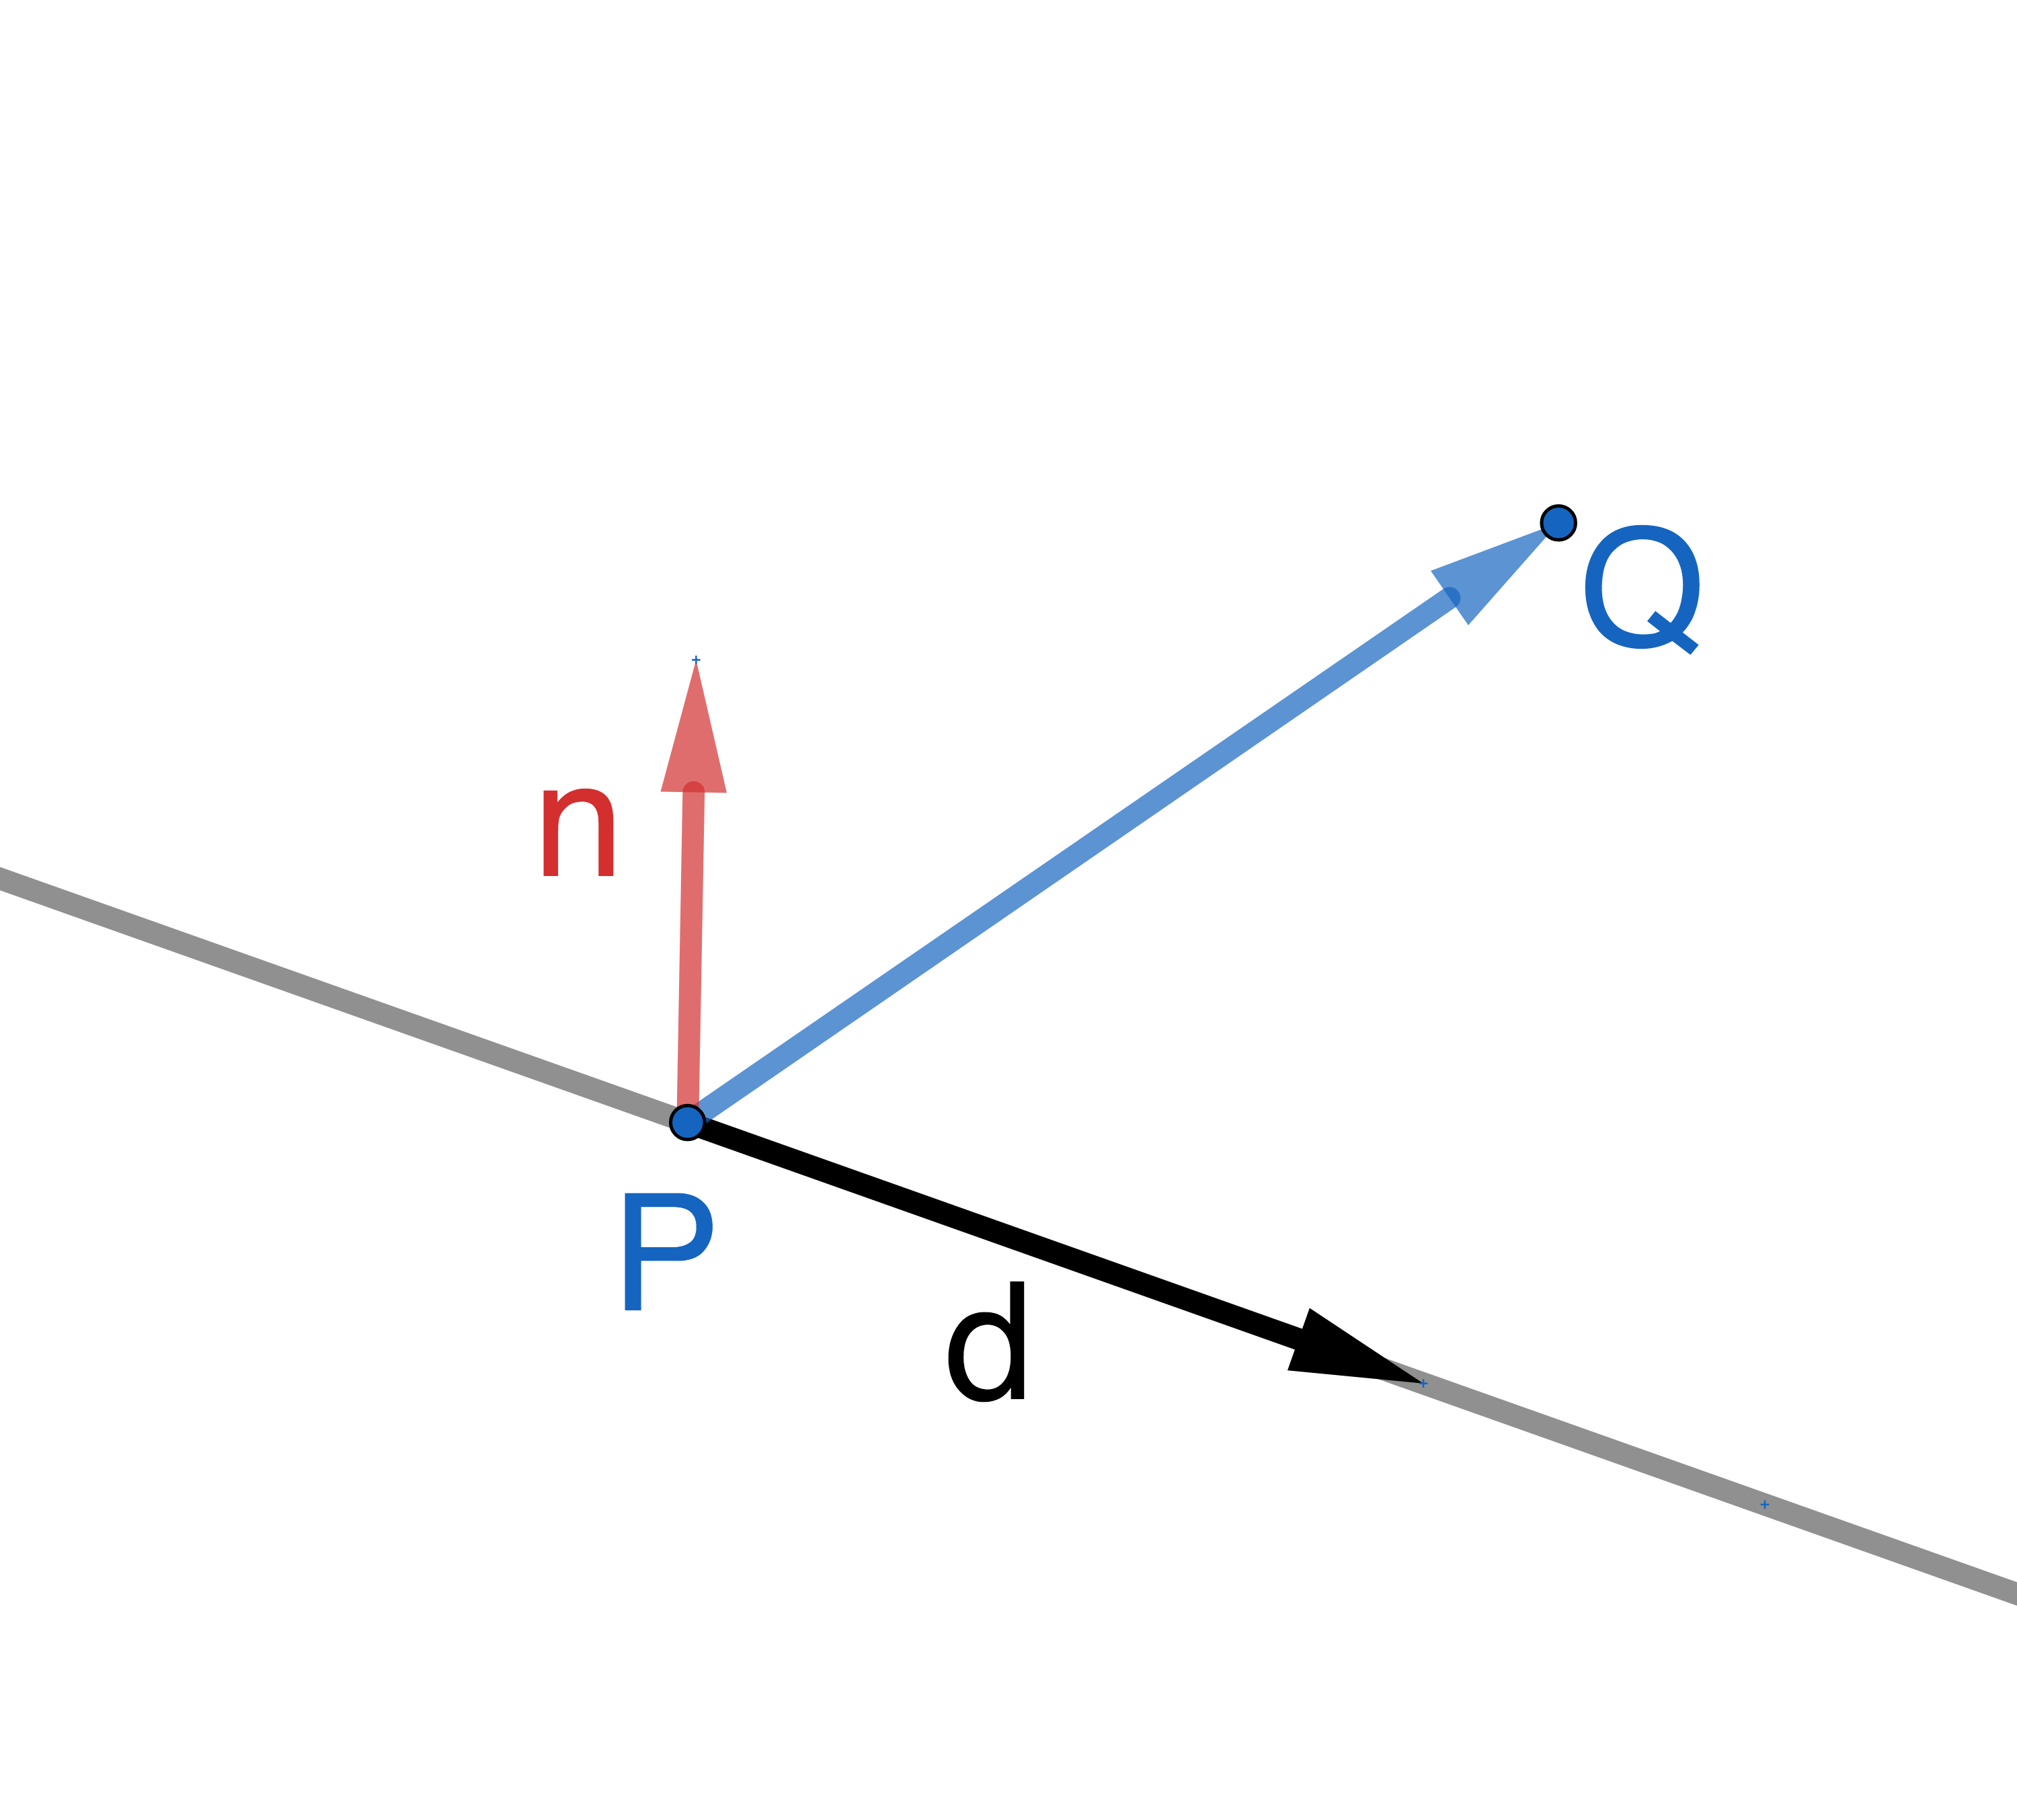
\includegraphics[scale=1.5]{plane-from-line-and-point.png}\\

  where the vector $n$ is any vector orthogonal to both $d$ and $\vec{QP}$.
  To find one such $n$ take the cross-product of $d$ and $\vec{QP}$:
  \begin{equation*}
  n = d\times (Q-P) = \left[
  \begin{array}{c}
  -2\\
  -2\\
  5
  \end{array}
  \right] \times \left[
  \begin{array}{c}
  -4\\
  1\\
  2
  \end{array}
  \right] = \left[
  \begin{array}{c}
  -4-5\\
  -20+4\\
  -2-8
  \end{array}
  \right] = \left[
  \begin{array}{c}
  -9\\
  -16\\
  -10
  \end{array}
  \right]
  \end{equation*}
  so the equation for the plane is
  \begin{align*}
    0 = n\cdot (x-P) &= \left[
    \begin{array}{c}
    -9\\
    -16\\
    -10
    \end{array}
    \right]\cdot \left[
    \begin{array}{c}
    x-9\\
    y+6\\
    z+1
    \end{array}
    \right] \\
    &= -9x +81 -16y-96 -10z -10\\
    & = -9x -16y -10z -25
  \end{align*}
  i.e. 
  \begin{equation*}
  9x+16y+10z = -25
  \end{equation*}
\end{Answer}

\begin{Exercise}
  Find a steady state vector for
  \begin{equation*}
  \left[
  \begin{array}{ccc}
  \frac{1}{2} & \frac{1}{4} & \frac{1}{4}\\
  0 & \frac{1}{2} & \frac{1}{4}\\
  \frac{1}{2} & \frac{1}{4} & \frac{1}{2}
  \end{array}
  \right]
  \end{equation*}
\end{Exercise}

\begin{Answer}
We need to solve:
  \begin{equation*}
  \left[
  \begin{array}{ccc|c}
  \frac{-1}{2} & \frac{1}{4} & \frac{1}{4}&0\\
  0 & \frac{-1}{2} & \frac{1}{4}&0\\
  \frac{1}{2} & \frac{1}{4} & \frac{-1}{2}&0
  \end{array}
  \right]
  \end{equation*}
  \begin{equation*}
  \rightarrow\left[
  \begin{array}{ccc|c}
  \frac{-1}{2} & \frac{1}{4} & \frac{1}{4}&0\\
  0 & \frac{-1}{2} & \frac{1}{4}&0\\
  0 & \frac{1}{2} & \frac{-1}{4}&0
  \end{array}
  \right]
  \end{equation*}
  \begin{equation*}
  \rightarrow\left[
  \begin{array}{ccc|c}
  1 & \frac{-1}{2} & \frac{-1}{2}&0\\
  0 & 1 & \frac{-1}{2}&0
  \end{array}
  \right]
  \end{equation*}
  \begin{equation*}
  \rightarrow\left[
  \begin{array}{ccc|c}
  1 & 0 & \frac{-3}{4}&0\\
  0 & 1 & \frac{-1}{2}&0
  \end{array}
  \right]
  \end{equation*}
  so $z = s$, $x = \frac{3s}{4}$ and $y = \frac{s}{2}$.
  \begin{equation*}
  E_1 = s \left[
  \begin{array}{c}
  \frac{3}{4}\\
  \frac{1}{2}\\
  1
  \end{array}
  \right] = \bar{s} \left[
  \begin{array}{c}
  3\\
  2\\
  4
  \end{array}
  \right]
  \end{equation*}
  therefore the steady state vector is
  \begin{equation*}
  \frac{1}{9} \left[
  \begin{array}{c}
  3\\
  2\\
  4
  \end{array}
  \right]
  \end{equation*}
  (i.e. choose $\bar{s}$ such that the entries sum to $1$.)
\end{Answer}

\begin{Exercise}
  If possible diagonalise
  \begin{equation*}
  \left[
  \begin{array}{ccc}
  3&-4&2\\
  1&-2&2\\
  1&-5&5
  \end{array}
  \right]
  \end{equation*}
\end{Exercise}

\begin{Answer}
  First find the eigenvalues:
  \begin{align*}
    det \left[
    \begin{array}{ccc}
    3\-\lambda & -4 & 2\\
    1& -2-\lambda & 2\\
    1 & -5 & 5-\lambda
    \end{array}
    \right] &= -det \left[
    \begin{array}{ccc}
    1 & -5 & 5-\lambda\\
    1& -2-\lambda & 2\\
    3\-\lambda & -4 & 2
    \end{array}
    \right] \\
    &= -det \left[
    \begin{array}{ccc}
    1 & -5 & 5-\lambda\\
    0& 3-\lambda & \lambda-3\\
    0 & 11-5\lambda & 2-(3-\lambda)(5-\lambda)
    \end{array}
    \right]\\
    &= (\lambda-3)det \left[
    \begin{array}{ccc}
    1 & -5 & 5-\lambda\\
    0& 1 & -1\\
    0 & 11-5\lambda & 2-(3-\lambda)(5-\lambda)
    \end{array}
    \right]\\
    &= (\lambda-3)det \left[
    \begin{array}{ccc}
    1 & -5 & 5-\lambda\\
    0& 1 & -1\\
    0 & 0 & 2-(3-\lambda)(5-\lambda)+11-5\lambda
    \end{array}
    \right] \\
    &= (\lambda -3)\left(2-(15-8\lambda +\lambda^2)+11-5\lambda\right)\\
    &= -(\lambda -3)(\lambda^2-3\lambda +2)\\
    &= (\lambda-3)(\lambda -1)(\lambda -2)
  \end{align*}
  The eigenspace associated to $1$:
  \begin{equation*}
  \left[
  \begin{array}{ccc|c}
  2&-4&2&0\\
  1&-3&2&0\\
  1&-5&4&0
  \end{array}
  \right]
  \end{equation*}
  \begin{equation*}
  \rightarrow\left[
  \begin{array}{ccc|c}
  1&-2&1&0\\
  1&-3&2&0\\
  1&-5&4&0
  \end{array}
  \right]
  \end{equation*}
  \begin{equation*}
  \rightarrow\left[
  \begin{array}{ccc|c}
  1&-2&1&0\\
  0&-1&1&0\\
  0&-3&3&0
  \end{array}
  \right]
  \end{equation*}
  \begin{equation*}
  \rightarrow\left[
  \begin{array}{ccc|c}
  1&-2&1&0\\
  0&1&-1&0\\
  \end{array}
  \right]
  \end{equation*}
  \begin{equation*}
  \rightarrow\left[
  \begin{array}{ccc|c}
  1&0&-1&0\\
  0&1&-1&0\\
  \end{array}
  \right]
  \end{equation*}
  and so the eigenspace is
  \begin{equation*}
  E_1 = s \left[
  \begin{array}{c}
  1\\
  1\\
  1
  \end{array}
  \right]
  \end{equation*}
  The eigenspace associated to $2$:
  \begin{equation*}
  \left[
  \begin{array}{ccc|c}
  1&-4&2&0\\
  1&-4&2&0\\
  1&-5&3&0
  \end{array}
  \right]
  \end{equation*}
  \begin{equation*}
  \rightarrow\left[
  \begin{array}{ccc|c}
  1&-4&2&0\\
  1&-5&3&0
  \end{array}
  \right]
  \end{equation*}
  \begin{equation*}
  \rightarrow\left[
  \begin{array}{ccc|c}
  1&-4&2&0\\
  0&-1&1&0
  \end{array}
  \right]
  \end{equation*}
  \begin{equation*}
  \rightarrow\left[
  \begin{array}{ccc|c}
  1&-4&2&0\\
  0&1&-1&0
  \end{array}
  \right]
  \end{equation*}
  \begin{equation*}
  \rightarrow\left[
  \begin{array}{ccc|c}
  1&0&-2&0\\
  0&1&-1&0
  \end{array}
  \right]
  \end{equation*}
  and so the eigenspace is:
  \begin{equation*}
  E_2 = s \left[
  \begin{array}{c}
  2\\
  1\\
  1
  \end{array}
  \right]
  \end{equation*}
  The eigenspace associated to $3$:
  \begin{equation*}
  \left[
  \begin{array}{ccc|c}
  0&-4&2&0\\
  1&-5&2&0\\
  1&-5&2&0
  \end{array}
  \right]
  \end{equation*}
  \begin{equation*}
  \rightarrow\left[
  \begin{array}{ccc|c}
  1&-5&2&0\\
  0&-4&2&0
  \end{array}
  \right]
  \end{equation*}
  \begin{equation*}
  \rightarrow\left[
  \begin{array}{ccc|c}
  1&-5&2&0\\
  0&1&\frac{-1}{2}&0
  \end{array}
  \right]
  \end{equation*}
  \begin{equation*}
  \rightarrow\left[
  \begin{array}{ccc|c}
  1&0&\frac{-1}{2}&0\\
  0&1&\frac{-1}{2}&0
  \end{array}
  \right]
  \end{equation*}
  so the eigenspace is
  \begin{equation*}
  E_3 = s \left[
  \begin{array}{c}
  1\\
  1\\
  2
  \end{array}
  \right]
  \end{equation*}
  Now for all of the eigenvalues ($1$, $2$ and $3$) the algebraic multiplicities are equal to the geometric multiplicities the matrix is diagonalisable. The diagonalising matrix is 
  \begin{equation*}
  P = \left[
  \begin{array}{ccc}
  1& 2 & 1\\
  1& 1& 1\\
  1& 1 &2
  \end{array}
  \right]
  \end{equation*}
  with corresponding diagonal matrix
  \begin{equation*}
  D = \left[
  \begin{array}{ccc}
  1 & 0 & 0\\
  0&2&0\\
  0&0&3
  \end{array}
  \right]
  \end{equation*}
\end{Answer}

\shipoutAnswer

\bibliography{references}
\bibliographystyle{hplain}

\end{document}
